\documentclass[xcolor=pdflatex,dvipsnames,table]{beamer}
\usepackage{epsfig,graphicx}
\usepackage{palatino}
\usepackage{fancybox}
\usepackage{relsize}
\usepackage[procnames]{listings}
\usepackage{hyperref}
\usepackage{qtree} % needed?
\usepackage{booktabs}
\usepackage{dirtree}
\usepackage[normalem]{ulem}


% fatter TT font
\renewcommand*\ttdefault{txtt}
% another TT, suggested by Alex
% \usepackage{inconsolata}
% \usepackage[T1]{fontenc} % needed as well?


\newcommand{\scale}{0.7}

\newcommand{\todo}[1]{{\emph{TODO: #1}}}
\newcommand{\martin}[1]{{\color{blue} Martin: #1}}
\newcommand{\abcdef}[1]{{\color{red} Author2: #1}}

% uncomment following for final submission
%\renewcommand{\todo}[1]{}
%\renewcommand{\martin}[1]{}
%\renewcommand{\author2}[1]{}

\newcommand{\code}[1]{{\texttt{#1}}}

\hypersetup{
  linkcolor  = black,
%  citecolor  = blue,
  urlcolor   = blue,
  colorlinks = true,
}

\beamertemplatenavigationsymbolsempty
\setbeamertemplate{footline}[frame number]





\newif\ifbook
% shared in slides and book

\lstdefinelanguage{chisel}{
  morekeywords={abstract,case,catch,class,def,%
    do,else,extends,false,final,finally,%
    for,if,implicit,import,match,mixin,%
    new,null,object,override,package,%
    private,protected,requires,return,sealed,%
    super,this,throw,trait,true,try,%
    type,val,var,while,with,yield},
  otherkeywords={=>,<-,<\%,<:,>:,\#,@},
  sensitive=true,
  morecomment=[l]{//},
  morecomment=[n]{/*}{*/},
  morestring=[b]",
  morestring=[b]',
  morestring=[b]"""
}

\usepackage{color}
\definecolor{dkgreen}{rgb}{0,0.6,0}
\definecolor{gray}{rgb}{0.5,0.5,0.5}
\definecolor{mauve}{rgb}{0.58,0,0.82}

% Default settings for code listings
\ifbook
\lstset{%frame=lines,
  language=chisel,
  aboveskip=3mm,
  belowskip=3mm,
  showstringspaces=false,
  columns=fixed, % basewidth=\mybasewidth,
  basicstyle={\small\ttfamily},
  numbers=none,
  numberstyle=\footnotesize,
  % identifierstyle=\color{red},
  breaklines=true,
  breakatwhitespace=true,
  procnamekeys={def, val, var, class, trait, object, extends},
  % procnamestyle=\ttfamily,
  tabsize=2,
  float
}
\else
\lstset{%frame=lines,
  language=chisel,
  aboveskip=3mm,
  belowskip=3mm,
  showstringspaces=false,
  columns=fixed, % basewidth=\mybasewidth,
  basicstyle={\small\ttfamily},
  numbers=none,
  numberstyle=\footnotesize\color{gray},
  % identifierstyle=\color{red},
  keywordstyle=\color{blue},
  commentstyle=\color{dkgreen},
  stringstyle=\color{mauve},
  breaklines=true,
  breakatwhitespace=true,
  procnamekeys={def, val, var, class, trait, object, extends},
  procnamestyle=\ttfamily\color{red},
  tabsize=2,
  float
}
\fi

\lstnewenvironment{chisel}[1][]
{\lstset{language=chisel,#1}}
{}

\newcommand{\shortlist}[1]{{\lstinputlisting[nolol]{#1}}}

\newcommand{\longlist}[3]{{\lstinputlisting[float, caption={#2}, label={#3}, frame=tb, captionpos=b]{#1}}}

\newcommand{\verylonglist}[3]{{\lstinputlisting[caption={#2}, label={#3}, frame=tb, captionpos=b]{#1}}}


\title{Testing and Verification}
\author{Martin Schoeberl}
\date{\today}
\institute{Technical University of Denmark\\
Embedded Systems Engineering}

\begin{document}

\begin{frame}
\titlepage
\end{frame}


\begin{frame}[fragile]{TODO}
\begin{itemize}
\item Midterm evaluation
\item \url{https://forms.gle/wtvDrA4peD4oLvt16}
\item Show ab solutions for last week
\item Show lab exercise 7-segment decoder
\item Also have the shift register (after some repetition)
\item  * link is missing: use simple bash scripts or Makefiles to remember commands (show examples)
\end{itemize}
\end{frame}


\begin{frame}[fragile]{Generating Timing with Counters}
\begin{itemize}
\item Generate a \code{tick} at a lower frequency
\item E.g., used for driving the display multiplexing at 1~kHz
\end{itemize}
\begin{figure}
  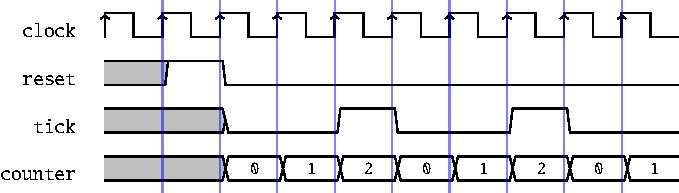
\includegraphics[scale=0.8]{../figures/tick_wave}
\end{figure}
\end{frame}


\begin{frame}[fragile]{The Tick Generation}
\shortlist{../code/sequ_tick_gen.txt}
\end{frame}

\begin{frame}[fragile]{Using the Tick}
\begin{itemize}
\item A counter running at a \emph{slower frequency}
\item By using the \code{tick} as an enable signal
\end{itemize}
\shortlist{../code/sequ_tick_counter.txt}
\end{frame}

\begin{frame}[fragile]{The \emph{Slow} Counter}
\begin{itemize}
\item Increment every \code{tick}
\end{itemize}
\begin{figure}
  \includegraphics[scale=0.8]{../figures/tick_count_wave}
\end{figure}
\end{frame}

\begin{frame}[fragile]{A Timer}
\begin{itemize}
\item Like a kitchen timer
\item Start by loading a timeout value
\item Count down till 0
\item Assert \code{done} when finished
\end{itemize}
\end{frame}

\begin{frame}[fragile]{One-Shot Timer}
\begin{figure}
  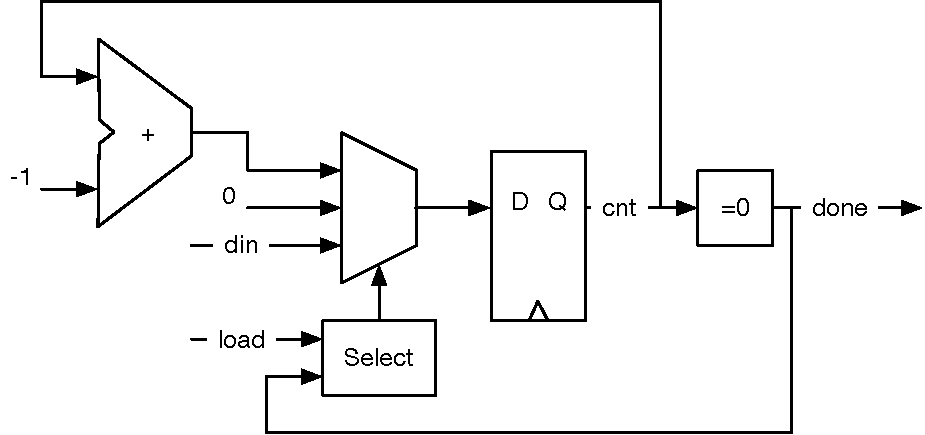
\includegraphics[scale=\scale]{../figures/timer}
\end{figure}
\end{frame}

\begin{frame}[fragile]{One-Shot Timer}
\shortlist{../code/timer.txt}
\end{frame}

\begin{frame}[fragile]{Summary on Counters}
\begin{itemize}
\item Counters are versatile tools
\item Count events
\item Generate timing ticks
\item Generate a one-shot timer
\end{itemize}
\end{frame}



\begin{frame}[fragile]{Chisel VHDL Comparison}
\begin{columns}
\column{0.5\textwidth}
\begin{chisel}
class DecodeExecute extends Bundle {
  val rs1 = UInt(32.W)
  val rs2 = UInt(32.W)
  val immVal = UInt(32.W)
  val aluOp = new AluOp()
}
\end{chisel}
\column{0.5\textwidth}
\begin{verbatim}
VHDL code here
\end{verbatim}
\end{columns}
Also show latch and and using a button as clock
\end{frame}

\begin{frame}[fragile]{Below Stuff Moved Over}
\begin{itemize}
\item From tutorial
\item Maybe used in the future
\end{itemize}
\end{frame}

\begin{frame}[fragile]{A Collection of Signals with \code{Vec}}
\begin{itemize}
\item Chisel \code{Vec} is a collection of signals of the same type
\item The collection can be accessed by an index
\item Similar to an array in other languages
\end{itemize}
\shortlist{../code/vec.txt}
\end{frame}

\begin{frame}[fragile]{Using a \code{Vec}}
\shortlist{../code/vec_access.txt}
\begin{itemize}
\item Reading from an \code{Vec} is a multplexer
\item We can put a \code{Vec} into a \code{Reg}
\end{itemize}
\shortlist{../code/reg_file.txt}
\noindent An element of that register file is accessed with an index and used as a normal register.

\shortlist{../code/reg_file_access.txt}
\end{frame}


\begin{frame}[fragile]{Mixing Vecs and Bundles}
\begin{itemize}
\item We can freely mix bundles and vectors
\item When creating a vector with a bundle
type, we need to pass a prototype for the vector fields. Using our
\code{Channel}, which we defined above, we can create a vector of channels with:
\end{itemize}
\shortlist{../code/vec_bundle.txt}
\begin{itemize}
\item A bundle may as well contain a vector
\end{itemize}
\shortlist{../code/bundle_vec.txt}
\end{frame}

\begin{frame}[fragile]{Add the following as new material to the repetition of the component/IO stuff}
\end{frame}

\begin{frame}[fragile]{Port Directions}
\begin{itemize}
\item Can be reversed with the \code{Flipped}
\item Convenient to have one bundle definition working as source
and destination used between two modules
\end{itemize}
\begin{chisel}
class Channel extends Bundle {
  val data = Input(UInt(32.W))
  val ready = Output(Bool())
  val valid = Input(Bool())
}

class ChannelUsage extends Bundle {
  val input = new Channel()
  val output = Flipped(new Channel())
}
\end{chisel}
\end{frame}

\begin{frame}[fragile]{Port Directions}
\begin{itemize}
\item Can be assigned at instantiation
\end{itemize}
\begin{chisel}
class ExecuteIO extends Bundle {
  val dec = Input(new DecodeExecute())
  val mem = Output(new ExecuteMemory())
}
\end{chisel}
\begin{chisel}
\end{chisel}
\end{frame}

\begin{frame}[fragile]{Connections}
\begin{itemize}
\item Simple connections just with assignments, e.g.,
\begin{chisel}
  adder.io.a := ina
  adder.io.b := inb
\end{chisel}
\item Automatic bulk connections between components
\begin{chisel}
  dec.io <> exe.io
  mem.io <> exe.io
\end{chisel}
\end{itemize}
\end{frame}

\begin{frame}[fragile]{Functional Abstraction}
\begin{chisel}
  def addSub(add: Bool, a: UInt, b: UInt) =
    Mux(add, a+b, a-b)

  val res = addSub(cond, a, b)
  
  def rising(d: Bool) = d && !RegNext(d)
\end{chisel}
\begin{itemize}
\item Functions for repeated pieces of logic
\item May contain state
\item Functions may return \emph{hardware}
\end{itemize}
\end{frame}

\begin{frame}[fragile]{Component Generation}
\begin{chisel}
val cores = new Array[Module](32)

for (j <- 0 until 32)
  cores(j) = Module(new CPU())
\end{chisel}
\begin{itemize}
\item Use Scala array to collect components
\item Generation with a Scala loop
\end{itemize}
\end{frame}

\begin{frame}[fragile]{Conditional Component Generation}
\begin{chisel}
val icache =
  if (TYPE == METHOD)
    Module(new MCache())
  else if (TYPE == LINE)
    Module(new ICache())
  else
    ChiselError.error("Unsupported Type")
\end{chisel}
\begin{itemize}
\item Use Scala if/else for conditional component types
\item Code example from Patmos
\item We parse an XML file for the configuration
\end{itemize}
\end{frame}

\begin{frame}[fragile]{Logic Generation}
\begin{itemize}
\item Read a file into a table
\begin{itemize}
\item E.g., to read in ROM content for a processor
\end{itemize}
\item Generate a truth table algorithmically
\begin{itemize}
\item E.g., generate binary to BCD translation
\end{itemize}
\item Use the full power of Scala
\end{itemize}
\begin{chisel}
val byteArray = Files.readAllBytes(Paths.get(fileName))
val arr = new Array[Bits](byteArray.length)
for (i <- 0 until byteArray.length) {
  arr(i) = Bits(byteArray(i), 8)
}
val rom = Vec[Bits](arr)
\end{chisel}
\end{frame}
%%%%%%%%%%%%%%%%%
%\begin{frame}[fragile]{zzz}
%\begin{chisel}
%code
%\end{chisel}
%\begin{itemize}
%\item xxx
%\item xxx
%\item xxx
%\end{itemize}
%\end{frame}
%
%\begin{frame}[fragile]{yyy}
%\begin{itemize}
%\item xxx
%\item xxx
%\item xxx
%\item xxx
%\item xxx
%\end{itemize}
%\end{frame}
%%%%%%%%%%%%%%%%%

\begin{frame}[fragile]{Scala Values and Variables}
\begin{chisel}
// A value is a constant
val i = 0
// No new assignment; this will not compile
i = 3

// A variable can change the value
var v = "Hello"
v = "Hello World"

// Type usually inferred, but can be declared
var s: String = "abc"
\end{chisel}
\end{frame}

\begin{frame}[fragile]{Simple Loops}
\begin{chisel}
// Loops from 0 to 9
// Automatically creates loop value i
for (i <- 0 until 10) {
  println(i)
}
\end{chisel}
\end{frame}

\begin{frame}[fragile]{Conditions}
\begin{chisel}
for (i <- 0 until 10) {
  if (i%2 == 0) {
    println(i + " is even")
  } else {
    println(i + " is odd")
  }
}
\end{chisel}
\end{frame}

\begin{frame}[fragile]{Scala Arrays and Lists}
\begin{chisel}
// An integer array with 10 elements
val numbers = new Array[Integer](10)
for (i <- 0 until numbers.length) {
  numbers(i) = i*10
}
println(numbers(9))


// List of integers
val list = List(1, 2, 3)
println(list)
// Different form of list construction
val listenum = 'a' :: 'b' :: 'c' :: Nil
println(listenum)
\end{chisel}
\end{frame}


\begin{frame}[fragile]{Scala Classes}
\begin{chisel}
// A simple class
class Example {
  // A field, initialized in the constructor
  var n = 0
  
  // A setter method
  def set(v: Integer) = {
    n = v
  }
  
  // Another method
  def print() = {
    println(n)
  }
}
\end{chisel}
\end{frame}

\begin{frame}[fragile]{Scala (Singleton) Object}
\begin{chisel}
object Example {}
\end{chisel}
\begin{itemize}
\item For \emph{static} fields and methods
\begin{itemize}
\item Scala has no static fields or methods like Java
\end{itemize}
\item Needed for \code{main}
\item Useful for helper functions
\end{itemize}
\end{frame}

\begin{frame}[fragile]{Singleton Object for the \code{main}}
\begin{chisel}
// A singleton object
object Example {
  
  // The start of a Scala program
  def main(args: Array[String]): Unit = {
    
    val e = new Example()
    e.print()
    e.set(42)
    e.print()
  }
}
\end{chisel}
\begin{itemize}
\item Compile and run it with sbt (or within Eclipse/IntelliJ):
\end{itemize}
\begin{chisel}
sbt "runMain Example"
\end{chisel}
\end{frame}

\begin{frame}[fragile]{Functions}
\begin{itemize}
\item Circuits can be encapsulated in functions
\item Each \emph{function call} generates hardware
\item Simple functions can be a single line
\end{itemize}
\begin{chisel}
  def adder(v1: UInt, v2: UInt) = v1 + v2
  
  val add1 = adder(a, b)
  val add2 = adder(c, d)
\end{chisel}
\end{frame}

\begin{frame}[fragile]{More Function Examples}
\begin{itemize}
\item Functions can also contain registers
\end{itemize}
\begin{chisel}
  def addSub(add: Bool, a: UInt, b: UInt) =
    Mux(add, a + b, a - b)

  val res = addSub(cond, a, b)

  def rising(d: Bool) = d && !RegNext(d)

  val edge = rising(cond)
\end{chisel}
\end{frame}

\begin{frame}[fragile]{The Counter as a Function}
\begin{itemize}
\item Longer functions in curly brackets
\item Last value is the return value
\end{itemize}
\begin{chisel}
def counter(n: UInt) = {
  
  val cntReg = RegInit(0.U(8.W))
  
  cntReg := cntReg + 1.U
  when(cntReg === n) {
    cntReg := 0.U
  }
  cntReg
}

val counter100 = counter(100.U)
\end{chisel}
\end{frame}


\begin{frame}[fragile]{Functions}
\begin{itemize}
\item Example from Patmos execute stage
\end{itemize}
\begin{chisel}
def alu(func: Bits, op1: UInt, op2: UInt): Bits = {
  val result = UInt(width = DATA_WIDTH)
  // some more lines...
  switch(func) {
    is(FUNC_ADD) { result := sum }
    is(FUNC_SUB) { result := op1 - op2 }
    is(FUNC_XOR) { result := (op1 ^ op2).toUInt }
    // some more lines
  }
  result
}
\end{chisel}
\end{frame}

\begin{frame}[fragile]{Scala List for Enumeration}
\begin{chisel}
  val empty :: full :: Nil = Enum(2)
\end{chisel}
\begin{itemize}
\item Can be used in wires and registers
\item Symbols for a state machine
\end{itemize}
\end{frame}

\begin{frame}[fragile]{Finite State Machine}
\begin{chisel}
  val empty :: full :: Nil = Enum(2)
  val stateReg = RegInit(empty)
  val dataReg = RegInit(0.U(size.W))

  when(stateReg === empty) {
    when(io.enq.write) {
      stateReg := full
      dataReg := io.enq.din
    }
  }.elsewhen(stateReg === full) {
    when(io.deq.read) {
      stateReg := empty
    }
  }
\end{chisel}
\begin{itemize}
\item A simple buffer for a bubble FIFO
\end{itemize}
\end{frame}

\begin{frame}[fragile]{Parameterization}
\begin{chisel}
class ParamChannel(n: Int) extends Bundle {
  val data = Input(UInt(n.W))
  val ready = Output(Bool())
  val valid = Input(Bool())
}

val ch32 = new ParamChannel(32)
\end{chisel}
\begin{itemize}
\item Bundles and modules can be parametrized
\item Pass a parameter in the constructor
\end{itemize}

\end{frame}
\begin{frame}[fragile]{A Module with a Parameter}
\begin{chisel}
class ParamAdder(n: Int) extends Module {
  val io = IO(new Bundle {
    val a = Input(UInt(n.W))
    val b = Input(UInt(n.W))
    val result = Output(UInt(n.W))
  })

  val addVal = io.a + io.b
  io.result := addVal
}

val add8 = Module(new ParamAdder(8))
\end{chisel}
\begin{itemize}
\item Parameter can also be a Chisel type
\item Can also be a generic type:
\item \code{class Mod[T <: Bits](param: T) extends...}
\end{itemize}
\end{frame}

\begin{frame}[fragile]{Scala \code{for} Loop for Circuit Generation}
\begin{chisel}
val shiftReg = RegInit(0.U(8.W))

shiftReg(0) := inVal

for (i <- 1 until 8) {
  shiftReg(i) := shiftReg(i-1)
}
\end{chisel}
\begin{itemize}
\item \code{for} is Scala
\item This loop generates several connections
\item The connections are parallel hardware
\end{itemize}
\end{frame}

\begin{frame}[fragile]{Conditional Circuit Generation}
\begin{chisel}
class Base extends Module { val io = new Bundle() }
class VariantA extends Base { }
class VariantB extends Base { }

val m = if (useA) Module(new VariantA())
        else Module(new VariantB())
\end{chisel}
\begin{itemize}
\item \code{if} and \code{else} is Scala
\item \code{if} is an expression that returns a value
\begin{itemize}
\item Like ``\code{cond ? a : b;}'' in C and Java
\end{itemize}
\item This is not a hardware multiplexer
\item Decides which module to generate
\item Could even read an XML file for the configuration
\end{itemize}
\end{frame}

%\begin{frame}[fragile]{Chisel has a Multiplexer}
\begin{figure}
  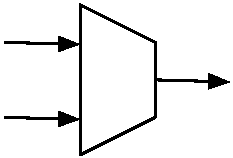
\includegraphics[scale=\scale]{../figures/mux}
\end{figure}
\shortlist{../code/mux.txt}
\begin{itemize}
\item So what?
\item Wait... What type is \code{a} and \code{b}?
\begin{itemize}
\item Can be any Chisel type!
\end{itemize}
\end{itemize}
\end{frame}

\begin{frame}[fragile]{Chisel has a Multiplexer}
\begin{figure}
  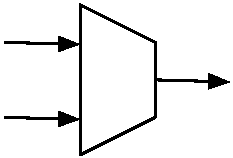
\includegraphics[scale=\scale]{../figures/mux}
\end{figure}
\shortlist{../code/mux.txt}
\begin{itemize}
\item SW people may not be impressed
\item They have generics since Java 1.5 in 2004
\begin{itemize}
\item \code{List<Flowers> != List<Cars>}
\end{itemize}
\end{itemize}
\end{frame}


\begin{frame}[fragile]{Generics in Hardware Construction}
\begin{itemize}
\item Chisel supports generic classes with type parameters
\item Write hardware generators independent of concrete type
\item This is a multiplexer \emph{generator}
\end{itemize}
\shortlist{../code/param_func.txt}
\end{frame}

\begin{frame}[fragile]{Put Generics Into Use}
\begin{itemize}
\item Let us implement a generic FIFO
\item Use the generic ready/valid interface from Chisel
\end{itemize}
\shortlist{../code/fifo_decoupled.txt}
\end{frame}

\begin{frame}[fragile]{Define the FIFO Interface}
\shortlist{../code/fifo_io.txt}
\begin{itemize}
\item We need enqueueing and dequeueing ports
\item Note the \code{Flipped}
\begin{itemize}
\item No more double definition of an interface
\end{itemize}
\end{itemize}
\end{frame}

\begin{frame}[fragile]{But What FIFO Implementation?}
\begin{itemize}
\item Bubble FIFO (good for low data rate)
\item Double buffer FIFO (fast restart)
\item FIFO with memory and pointers (for larger buffers)
\begin{itemize}
\item Using flip-flops
\item Using on-chip memory
\end{itemize}
\item And some more...
\end{itemize}
\begin{itemize}
\item This calls for object-oriented \sout{programming} \emph{hardware construction}
\end{itemize}
\end{frame}

\begin{frame}[fragile]{Abstract Base Class}
\shortlist{../code/fifo_abstract.txt}
\begin{itemize}
\item May contain common code
\item Extend by concrete classes
\end{itemize}
\begin{chisel}
class BubbleFifo[T <: Data](gen: T, depth: Int) extends Fifo(gen: T, depth: Int) {
\end{chisel}
\end{frame}



\begin{frame}[fragile]{Select a Concrete FIFO Implementation}
\begin{itemize}
\item Decide at hardware generation
\item Can use all Scala/Java power for the decision
\begin{itemize}
\item Connect to a web service, get \sout{Google} Alphabet stock price, and decide on which to use ;-)
\item For sure a silly idea, but you see what is possible...
\item Developers may find clever use of the Scala/Java power
\item We could present a GUI to the user to select from
\end{itemize}
\item We use XML files parsed at hardware generation time
\item End of TCL, Python,... generated hardware
\end{itemize}
\end{frame}

\begin{frame}[fragile]{Binary to BCD Conversion for VHDL}
\begin{figure}
    \centering
    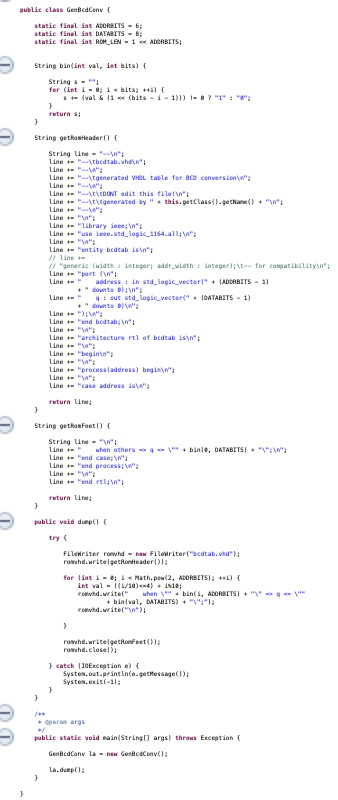
\includegraphics[scale=0.6]{JavaBCD}
\end{figure}
\end{frame}

\begin{frame}[fragile]{Java Program}
\begin{itemize}
\item Generates a VHDL table
\item The core code is:
\end{itemize}
\begin{chisel}
for (int i = 0; i < Math.pow(2, ADDRBITS); ++i) {
    int val = ((i/10)<<4) + i%10;
    // write out VHDL code for each line
\end{chisel}
\begin{itemize}
\item With all boilerplate 118 LoC
\end{itemize}
\end{frame}

\begin{frame}[fragile]{Chisel Version of Binary to BCD Conversion}
\begin{chisel}
  val array = new Array[Int](256)
  for (i <- 0 to 99) {
    array(i) = ((i/10)<<4) + i%10
  }
  val table = VecInit(array.map(_.U(8.W)))
\end{chisel}
\begin{itemize}
\item Directly generates the hardware (\code{VecInit})
\end{itemize}
\end{frame}

\begin{frame}[fragile]{Use Functional Programming for Generators}
\shortlist{../code/fun_first.txt}
\shortlist{../code/fun_func_lit.txt}
\shortlist{../code/fun_reduce_tree.txt}
\begin{itemize}
\item This is a simple example
\item What about an arbiter tree with fair arbitration?
\end{itemize}
\end{frame}

%\begin{frame}[fragile]{XXX}
%\begin{itemize}
%\item TODO: s4noc connection is part of the generator story
%\item
%\item
%\end{itemize}
%\end{frame}
%
%\begin{frame}[fragile]{XXX}
%\begin{itemize}
%\item
%\item
%\item
%\end{itemize}
%\end{frame}



\begin{frame}[fragile]{Generation Slides (inlude) are missing here}
\begin{itemize}
\item 
\end{itemize}
\end{frame}

\begin{frame}[fragile]{Combinational (Truth) Table Generation}
\begin{chisel}
val arr = new Array[Bits](length)
for (i <- 0 until length) {
  arr(i) = ...
}
val rom = Vec[Bits](arr)
\end{chisel}
\begin{itemize}
\item Generate a table in a Scala array
\item Use that array as input for a Chisel \code{Vec}
\item Generates a logic table at hardware construction time
\end{itemize}
\end{frame}

\begin{frame}[fragile]{BCD Generation Example}
\begin{itemize}
\item Explain BCD with examples
\item Show code
\end{itemize}
\end{frame}

\begin{frame}[fragile]{Ideas for Runtime Table Generation}
\begin{itemize}
\item Assembler in Scala/Java generates the boot ROM
\item Table with a \code{sin} function
\item Binary to BCD conversion
\item Schedule table for a TDM based network-on-chip
\item 
\item More ideas?
\end{itemize}
\end{frame}

\begin{frame}[fragile]{Memory}
\begin{chisel}
val mem = Mem(Bits(width = 8), size)

// write
when(wrEna) {
  mem(wrAddr) := wrData
}

// read
val rdAddrReg = Reg(next = rdAddr)
rdData := mem(rdAddrReg)
\end{chisel}
\begin{itemize}
\item Write is synchronous
\item Read can be asynchronous or synchronous
\item But there are no asynchronous memories in an FPGA
\end{itemize}
\end{frame}

\begin{frame}[fragile]{Factory Methods}
\begin{itemize}
\item Simpler component creation and use
\item Usage similar to built in components, such as \code{Mux}
\end{itemize}
\begin{chisel}
val myAdder = Adder(x, y)
\end{chisel}
\begin{itemize}
\item A little bit more work on component side
\item Define an \code{apply} method on the companion object that returns the component
\end{itemize}
\begin{chisel}
object Adder {
  def apply(a: UInt, b: UInt) = {
    val adder = Module(new Adder)
    adder.io.a := a
    adder.io.b := b
    adder.io.result
  }
}
\end{chisel}
\end{frame}

\begin{frame}[fragile]{Chisel and Scala}
\begin{itemize}
\item Chisel is a library written in Scala
\begin{itemize}
\item Import the library with \code{import chisel3.\_}
\end{itemize}
\item Chisel code is Scala code
\item When it is run is \emph{generates} hardware
\begin{itemize}
\item Verilog for synthesize
\item Scala netlist for simulation (testing)
\end{itemize}
\item Chisel is an embedded domain specific language
\item Two languages in one can be a little bit confusing
\end{itemize}
\end{frame}

\begin{frame}[fragile]{Scala}
\begin{itemize}
\item Is object oriented
\item Is functional
\item Strongly typed with very good type inference
\item Runs on the Java virtual machine
\item Can call Java libraries
\item Consider it as Java++
\begin{itemize}
\item Can almost be written like Java
\item With a more lightweight syntax
% \item Scala for Java Refugees is a nice tutorial (but link is dead)
% \item \url{http://www.codecommit.com/blog/scala/roundup-scala-for-java-refugees}
\end{itemize}
\end{itemize}
\end{frame}

\begin{frame}[fragile]{Scala Hello World}
\begin{chisel}
object HelloWorld extends App {
  println("Hello, World!")
}
\end{chisel}
\begin{itemize}
\item Compile with \code{scalac} and run with \code{scala}
\item You can even use Scala as scripting language
\item Show both
\end{itemize}
\end{frame}



\begin{frame}[fragile]{Generic Components}
\begin{chisel}
val c = Mux(cond, a, b)
\end{chisel}
\begin{itemize}
\item This is a multiplexer
\item Input can be any type
\end{itemize}
\end{frame}

\begin{frame}[fragile]{Testing}
\begin{chisel}
class CounterTester(c: Counter) extends PeekPokeTester(c) {
  for (i <- 0 until 5) {
    println(i.toString + ": " + peek(c.io.out).toString())
    step(1)
  }
}
\end{chisel}
\begin{itemize}
\item Within Chisel with a tester (= Scala program)
\item May include waveform generation
\item peek and poke to read and set values
\begin{itemize}
\item Remember the BASIC days ;-)
\end{itemize}
\item printf in simulation on rising edge
\begin{chisel}
printf("Counting %x\n", r1)
\end{chisel}
\end{itemize}
\end{frame}



\begin{frame}[fragile]{Scala Build Tool (sbt)}
\begin{itemize}
\item Downloads Scala compiler if needed
\item Downloads dependent libraries (e.g., Chisel)
\item Compiles Scala programs
\item Executes Scala programs
\item Does a lot of magic, maybe too much
\item Compile and run with:
\end{itemize}
\begin{chisel}
sbt "runMain simple.Example"
\end{chisel}
\begin{itemize}
\item Or even just:
\end{itemize}
\begin{chisel}
sbt run
\end{chisel}
\end{frame}

\begin{frame}[fragile]{Build Configuration}
\begin{itemize}
\item Defines needed Scala version
\item Library dependencies
\item File name: \code{build.sbt}
\end{itemize}
\begin{chisel}
scalaVersion := "2.11.7"

resolvers ++= Seq(
  Resolver.sonatypeRepo("snapshots"),
  Resolver.sonatypeRepo("releases")
)

libraryDependencies += "edu.berkeley.cs" %% "chisel3" % "3.1.2"
libraryDependencies += "edu.berkeley.cs" %% "chisel-iotesters" % "1.2.2"
\end{chisel}
\end{frame}


\begin{frame}[fragile]{What is a Minimal Chisel Project?}
\begin{itemize}
\item Scala class (e.g., \code{Hello.scala})
\item Build info in \code{build.sbt} for \code{sbt}:
\end{itemize}
\begin{chisel}
scalaVersion := "2.11.7"

libraryDependencies += "edu.berkeley.cs" %% "chisel3" % "3.1.2"
\end{chisel}
\begin{itemize}
\item Run the process manually (look into the Makefile)
\end{itemize}
\end{frame}




\begin{frame}[fragile]{Chisel Main for Testing}
\begin{itemize}
\item Tests can be written in Scala/Chisel
\item Tester and device under test (DUT) are two processes
\item Invoke \code{execute} with some parameters, the DUT, and a tester
\end{itemize}
\begin{chisel}
object CounterTester extends App {

  iotesters.Driver.execute(Array[String](), () => new Counter(2)) {
    c => new CounterTester(c)
  }
}
\end{chisel}
\end{frame}

\begin{frame}[fragile]{A Chisel Tester}
\begin{itemize}
\item Extends class \code{PeekPokeTester}
\item Has the DUT as parameter
\item Testing code can use all features of Scala
\end{itemize}
\begin{chisel}
class CounterTester(dut: Counter) extends PeekPokeTester(dut) {

  // Here comes the Chisel/Scala code
  // for the testing
}
\end{chisel}
\end{frame}

\begin{frame}[fragile]{Testing}
\begin{itemize}
\item Set input values with \code{poke}
\item Advance the simulation with \code{step}
\item Read the output values with \code{peek}
\item Compare the values with \code{expect}
\end{itemize}
\end{frame}

\begin{frame}[fragile]{Testing Example}
\begin{chisel}
// Set input values
poke(dut.io.a, 3)
poke(dut.io.b, 4)
// Execute one iteration
step(1)
// Print the result
val res = peek(dut.io.result)
println(res)

// Or compare against expected value
expect(dut.io.result, 7)
\end{chisel}
\end{frame}

\begin{frame}[fragile]{A Tiny ALU: IO Connection}
\begin{chisel}
class Alu extends Module {
  val io = IO(new Bundle {
    val fn = Input(UInt(2.W))
    val a = Input(UInt(4.W))
    val b = Input(UInt(4.W))
    val result = Output(UInt(4.W))
  })

  // Use shorter variable names
  val fn = io.fn
  val a = io.a
  val b = io.b
\end{chisel}
\end{frame}

\begin{frame}[fragile]{A Tiny ALU: The Function}
\begin{chisel}
  val result = Wire(UInt(4.W))
  // some default value is needed
  result := 0.U

  // The ALU selection
  switch(fn) {
    is(0.U) { result := a + b }
    is(1.U) { result := a - b }
    is(2.U) { result := a | b }
    is(3.U) { result := a & b }
  }

  // Output on the LEDs
  io.result := result
}
\end{chisel}
\end{frame}

\begin{frame}[fragile]{Testing the ALU}
\begin{itemize}
\item Compute the expected result in Scala
\end{itemize}
\begin{chisel}
  // This is exhaustive testing,
  // which usually is impossible
  for (a <- 0 to 15) {
    for (b <- 0 to 15) {
      for (op <- 0 to 3) {
        val result =
          op match {
            case 0 => a + b
            case 1 => a - b
            case 2 => a | b
            case 3 => a & b
          }
        val resMask = result & 0x0f
\end{chisel}

\end{frame}

\begin{frame}[fragile]{Testing the ALU}
\begin{itemize}
\item Compare the Scala computed result with the hardware result
\end{itemize}
\begin{chisel}
        poke(dut.io.fn, op)
        poke(dut.io.a, a)
        poke(dut.io.b, b)
        step(1)
        expect(dut.io.result, resMask)
      }
    }
  }
\end{chisel}
\end{frame}

\begin{frame}[fragile]{Generating Wave Forms}
\begin{itemize}
\item Additional parameters: \code{"--generate-vcd-output", "on"}
\item IO signals and registers are dumped
\item Option \code{--debug} puts all wires into the dump
\item Generates a .vcd file
\item Viewing with gtkwave or ModelSim
\item See the example with \code{make fifo}
\begin{itemize}
\item Show it
\end{itemize}
\item BubbleFifo contains also longer testing code
\end{itemize}
\end{frame}


\begin{frame}[fragile]{Summary}
\begin{itemize}
\item Chisel is a small language
\item Embedding it in Scala gives the power
\item We can write circuit generators
\item We can to co-simulation
\item We just scratched the surface
\end{itemize}
\end{frame}




\end{document}

